\documentclass[tikz,border=10pt]{standalone}
% Scale s = 0.009988 cm/px, centred on ink bbox (cx=457, cy=252); y flipped
\begin{document}
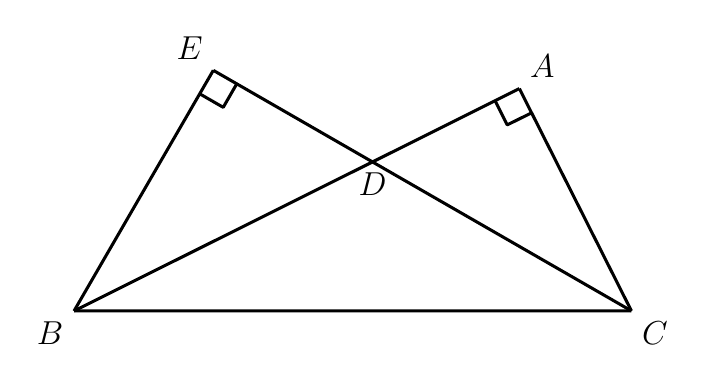
\begin{tikzpicture}[line width=1.1pt, line join=round]
  % Named vertices (converted from pixels)
  \coordinate (B) at (-3.534,-1.524);
  \coordinate (C) at (3.545,-1.523);
  \coordinate (D) at (0.257,0.370);
  \coordinate (A) at (2.122,1.300);
  \coordinate (E) at (-1.765,1.532);

  % Right-angle mark at A (corner square: arms A->P1, A->P3, far corner P2)
  \coordinate (PA1) at (1.813,1.147);
  \coordinate (PA2) at (1.968,0.839);
  \coordinate (PA3) at (2.276,0.992);

  % Right-angle mark at E
  \coordinate (QE1) at (-1.467,1.361);
  \coordinate (QE2) at (-1.639,1.062);
  \coordinate (QE3) at (-1.938,1.234);

  % Solid segments
  \draw (B) -- (C);
  \draw (B) -- (A);   % passes through D
  \draw (E) -- (C);   % passes through D
  \draw (E) -- (B);
  \draw (A) -- (C);

  % Right-angle marks (drawn inside the triangles)
  \draw (PA1) -- (PA2) -- (PA3);
  \draw (QE1) -- (QE2) -- (QE3);

  % Labels
  \node[above right] at (A) {\fontsize{11.5}{13.8}\selectfont $A$};
  \node[below left]  at (B) {\fontsize{11.5}{13.8}\selectfont $B$};
  \node[below right] at (C) {\fontsize{11.5}{13.8}\selectfont $C$};
  \node[below]       at (D) {\fontsize{11.5}{13.8}\selectfont $D$};
  \node[above left]  at (E) {\fontsize{11.5}{13.8}\selectfont $E$};
\end{tikzpicture}
\end{document}